\chapter{Proof on kinematic, shape, external forces and moments relations on deformable particle.}
\label{ap:cinematic}

    % \begin{align}
%     \phi\left<\bm{u}\right>^d 
%     &= n/\rho_d\left<\bm{p}_\alpha\right>^p
%     + \sum_{q=1}^\infty \left[\frac{(-1)^q}{q!} \prod^q_{i=1}\bm{\nabla} (n\left< \bm{Q}_\alpha^q\right>^p)\right]\\
%     \label{eq:exp}
% \end{align}
\tb{
\section{On the particles shape tensors for general to specific cases.}

All along the derivation of the averaged equations for the hybrid model we see appear this tensor : $\bm{\mathcal{G}_\alpha}^n = \int_{V_\alpha} \left(\bm{\bm{r}_\alpha}\right)^n dV$. 
In this Appendix we wish to give more physical sense to this tensor by taking the example of simple cases.
First, let's start with some basics.
For any shape the $0^{th}$ order of this tensor is the volume of the particle, it reads, $\bm{\mathcal{G}_\alpha}^0 = \int_{V_\alpha} dV = V_\alpha$.
For any particles the first order tensor $\bm{\mathcal{G}_\alpha}^0$ is always null, indeed by using the definition of  $\bm{r}_\alpha$ and $\bm{y}_\alpha$  it yields the following relation,
\begin{equation}
    \bm{\mathcal{G}_\alpha}^l
    = \int_{V_\alpha} \bm{r}_\alpha^n dV 
    = \int_{V_\alpha} \bm{y} dV - \bm{y}_\alpha \int  dV .
    = V_\alpha \bm{y}_\alpha - \bm{y}_\alpha V_\alpha 
    = 0.
\end{equation}
Then, in order to understand the meaning of the higher order tensor it is useful to think in terms of central moments and probability density function used in statistical theories. 
Therefore, the integral : $\int_{V_\alpha} \bm{r}_\alpha dV$, is equivalent to, 
\begin{equation}
    \mathcal{G}^n 
    = V_\alpha\int \bm{r}_\alpha^n f_\alpha(\bm{y}) d\bm{y},
\end{equation}
where $\bm{r}_\alpha = \bm{y}_\alpha -\bm{y}$, and $f_\alpha$ is a probability density function defined as such,
\begin{equation}
    f_\alpha(\bm{y}) = \left\{
        \begin{tabular}{cc}
        $1/V_\alpha \text{  if  }$ &$\bm{y}  \in V_\alpha$\\
        $0 \text{  if  }$ &$\bm{y} \notin  V_\alpha$
    \end{tabular}
    \right..
\end{equation}
Now we see clearly that $\mathcal{G}^n$ is the $n^{th}$ centered moment of the distribution of $f_\alpha$. 
Therefore, it follows that,
the first moment is the mean, i.e $\bm{y}_\alpha$. 
The second moment is variance, i.e. the spreading of the distribution computed by $\mathcal{G}^2$. 
The third moment is the skewness, it measures the asymmetry of the distribution, i.e. $\mathcal{G}^3$. 
The fourth moment is the Kurtosis, it measures the heaviness of the tail of the distribution, i.e. the shape. 

Some comment of the second order shape tensor are of interest. 
Indeed, it must respect some property, 

$\frac{d}{dt}\text{det}(\mathcal{G}) = 0$

to respect the pass conservation.
\subsection{2D disc shape tensor}

\tdplotsetmaincoords{70}{110}
%
\pgfmathsetmacro{\thetavec}{48.17}
\pgfmathsetmacro{\phivec}{63.5}
%
\begin{figure}[h!]
    \centering
    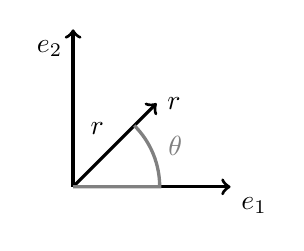
\begin{tikzpicture}[very thick]
        % \draw[fill=gray!30] (0,0)circle(1);
        \draw[->](0,0) --++ (2,0)node[below right ]{$\bm{e}_1$};
        \draw[->](0,0) --++ (0,2)node[below left ]{$\bm{e}_2$};
        \draw[->](0,0) --++ (45:1.5)node[right]{$r$}node[midway, above left]{$r$};
        \draw[gray](0,0) --++ (0:1.1)arc(0:45:1.1)node[below right]{$\;\;\;\theta$};
    \end{tikzpicture}   
	\begin{tikzpicture}[tdplot_main_coords,scale = 0.3]
		\draw[->,thick] (0,0,0) -- (6.5,0,0) node [pos=1.1] {$\bm{e}_1$};
		\draw[->,thick] (0,0,0) -- (0,6,0) node [pos=1.05] {$\bm{e}_2$};
		\draw[->,thick] (0,0,0) -- (0,0,5.5)  node [pos=1.05] {$\bm{e}_3$};   
		\tdplotsetcoord{P'}{7}{\thetavec}{\phivec}
    	\tdplotsetcoord{P''}{1}{90}{90+\phivec}
    	\tdplotsetcoord{P'''}{1}{90+\thetavec}{\phivec}
		\tdplotsetcoord{P}{6}{\thetavec}{\phivec}
		\draw[->] (0,0,0) -- (P) node [midway, above] {$r$};
		\draw[thick] (0,0,0) -- (2,4,0);
		\draw[dashed] (2,4,4) -- (2,4,0);
		\draw[dashed] (2,0,0) -- (2,4,0) node [pos=-0.1] {$x$};
		\draw[dashed] (0,4,0) -- (2,4,0) node [pos=-0.3] {$y$};
		\draw[dashed] (0,0,4) -- (2,4,4) node [pos=-0.1] {$z$};
		\draw[dashed, tdplot_main_coords] (4.47,0,0) arc (0:90:4.47);
		\node[fill=black, circle, inner sep=0.8pt] at (2,4,4) {};
		\tdplotdrawarc{(0,0,0)}{0.7}{0}{\phivec}{below}{$\phi$}
	    \tdplotsetthetaplanecoords{\phivec}
	    \tdplotdrawarc[tdplot_rotated_coords]{(0,0,0)}{0.5}{0}{\thetavec}{}{}
	    \node at (0,0.25,0.67) {$\theta$};
	\end{tikzpicture}

    \caption{Parametrization of the problem for 2D and 3D case.}
    \label{fig:schemeshpere}
\end{figure}
Now let's derive the first 4 moments for a 2D spherical particle. 
The zeroth moment reads as,
\begin{equation}
    \mathcal{G}^0 
    = \int_V  d\bm{y} 
    = \int_0^{2\pi}\int_0^{R}  d\bm{y} 
    = [\theta]_0^{2\pi}[r]_0^{R} 
    = 2\pi R
\end{equation}
where we used the notation depicted on the scheme \ref{fig:schemeshpere}.
The first moment as already mentioned is, $\mathcal{G}^1 = \int \bm{r}_\alpha dV = 0$.
Next, the second moment yields,
\begin{equation}
    (\mathcal{G}^2)_{ij}
    = \int_V r_ir_j d\bm{y} 
    = \int_0^{2\pi}\int_0^{R} r_ir_j d r dr d\theta 
    = \int_0^{R} r^3 dr \int_0^{2\pi} r_ir_j d\theta  
    = \frac{R^4}{4} \int_0^{2\pi} r_ir_j d\theta 
\end{equation}
where $\bm{r} = (\cos{\theta}, \sin{\theta})$. 
Then, 
\begin{equation}
    \mathcal{G}^2 = \frac{R^4}{4}\left[\begin{tabular}{cc}
        $\pi$&$0$\\
        $0$&$\pi$\\
    \end{tabular}
    \right].
\end{equation}
More generally the $l^{th}$ moment reads as, 
\begin{equation}
    (\mathcal{G}^l)_{i_1i_2\ldots i_l}
    = \frac{R^{l+2}}{l+2} \int_0^{2\pi} r_{i_1}r_{i_2}\ldots r_{i_l} d\theta 
\end{equation}
Then, two things can be shown. 
The first one, is that the components off-diagonal of $\mathcal{G}^l$ are null. 
The second, is that the values on the diagonal are the same. 
If we consider the sum on all indices, the product $r_{i_1}r_{i_2}\ldots r_{i_l}$ can be written $(\cos\theta+\sin\theta)^l$.
Moreover, 
\begin{equation}
    (\cos\theta+\sin\theta)^l  = \sum_{k=0}^l\binom{l}{k}\cos^k\theta\sin^{l-k}\theta
\end{equation}
Thus, the integral $\int_0^{2\pi} r_{i_1}r_{i_2}\ldots r_{i_l} d\theta$ always follows this form,
\begin{equation}
    \int_0^{2\pi} \cos^k\theta\sin^{l-k}\theta d\theta \;\;\;\forall k\leq l. 
    \label{eq:cossin}
\end{equation}
Now, we can notice that the diagonal components $I$ and $II$ (i.e. the diagonal in the sense that all the indices are the same) are equal to,
\begin{equation}
    (\mathcal{G}^l)_{I}
    = \int_0^{2\pi} \cos^l d\theta\;\;\;
    (\mathcal{G}^l)_{II}
    = \int_0^{2\pi} \sin^l d\theta  
\end{equation}
Let's develop the first term, 
\begin{align*}
    (\mathcal{G}^l)_{I}
    &= \int_0^{2\pi} \cos^l d\theta\\
    &= \frac{1}{l} \left[\cos^{l-1}\theta\sin\theta \right]_0^{2\pi} + \frac{l-1}{l} \int_0^{2\pi} \cos^{l-2} d\theta.\\
\end{align*}
The first term on the right hands side is always null. 
Indeed, $\cos$ is pair at any power of, $l-1$, and $\sin$ is odd, thus the product of the two terms is an odd function. 
Moreover, the product between $\sin$ or $\cos$ are at least $2\pi$ periodic. 
Therefore, the integral taken between $0$ and $\pi$ is null, and the relation reduce to, 
\begin{equation*}
    (\mathcal{G}^l)_{I}
    = \int_0^{2\pi} \cos^l d\theta
    =  \frac{l-1}{l} \int_0^{2\pi} \cos^{l-2} d\theta\\
    =  \frac{l-1}{l}\frac{l-3}{l-2} \int_0^{2\pi} \cos^{l-4} d\theta\\
\end{equation*}
If we keep repeating the process we eventually arrive to the smallest power. 
Which is either $0$ or $1$ if we start by, respectively a number $l$ pair and a number $l$ odd.
Therefore, we pose $l = 2q$ in the first case and $l = 2q+1$ in the second, 
\begin{equation*}
    (\mathcal{G}^{2q})_{I}
    =  \frac{2q-1}{2q}\frac{2q-3}{2q-2} \int_0^{2\pi} \cos^{2q-4}\theta d\theta\\
    =  \prod^{q-1}_{k= 0}\frac{2q-2k-1}{2q-2k} \int_0^{2\pi}  d\theta\\
    =  \prod^{q-1}_{k= 0}\frac{2q-2k-1}{2q-2k} 2\pi\\,
\end{equation*}
and,
\begin{equation*}
    (\mathcal{G}^{2q+1})_{I}
    =  \prod^{q}_{k= 0}\frac{2q-2k}{2q-2k+1} \int_0^{2\pi} \cos \theta d\theta\\
    = 0.
\end{equation*}
Similar calculation can be done for the powers of $\sin$, and it yields the same results. 
Therefore, the diagonal components of the $l^{th}$ order tensor of a disk are, 
\begin{equation}
    \mathcal{G}_{I}^l=\mathcal{G}_{II}^l = \left\{\begin{tabular}{cc}
        $\prod^{q-1}_{k= 0}\frac{2q-2k-1}{2q-2k} 2\pi $& if $l = 2q$     \\
        $0 $        & if $l = 2q+1$
    \end{tabular}\right.
    \label{eq:cosl}
\end{equation}
In fact, if we can carry out similar calculations for the integral, \ref{eq:cossin}, we find that, 
\begin{equation}
    \int_0^{2\pi} \sin^k \cos^{l-k} dV = \frac{1}{2}\frac{k-1}{l-k-1} \int_0^{2\pi} \sin^{l-2}\theta \cos^{l-k+2}\theta d\theta.
\end{equation}
Notice that taking $l = 2q$ or $l=2q+1$ leads to either $\sin^0\theta^{l-k+2q} $ or $\sin \theta^{l-k+2q+1}$ in the integral. 
Therefore, the integral of  $\sin \theta^{l-k+2q+1}$ between $0$ and $2\pi$ will ultimately cancel out. 
Therefore, we obtain the following relation in the non-null cases,
\begin{equation}
    \int_0^{2\pi} \sin^k \cos^{l-k} d\theta = \left\{\begin{tabular}{cc}
        $\prod^{q-1}_{n=0}\frac{2q-2n-1}{l-2q+2n+1} \int_0^{2\pi} \cos^{l} d\theta$& if $k = 2q$     \\
        $0 $        & if $l = 2q+1$
    \end{tabular}\right.
\end{equation}
Using \ref{eq:cosl} yields,
\begin{equation}
    \int_0^{2\pi} \sin^k \cos^{l-k} d\theta = \left\{\begin{tabular}{cc}
        $\prod^{q-1}_{n=0}\frac{2q-2n-1}{2r-2q+2n+1} \prod^{r-1}_{n= 0}\frac{2r-2n-1}{2r-2n} 2\pi $& if $k = 2q$ and $l = 2r$    \\
        $0$        & if $k = 2q  $ and $l = 2r +1$\\
        $0$        & if $k = 2q+1$ and $l = 2r$\\
        $0$        & if $k = 2q+1$ and $l = 2r +1$
    \end{tabular}\right.
\end{equation}
The remaining question is now, how to link the indexes of the tensor to the value of $k$.
If we consider a tensor of order $2$ it is easy to say that, 
\begin{equation}
    \mathcal{G}_{ij} = \delta_{ij} \frac{R^4}{4}\pi. 
\end{equation} 
For a $4^{th}$ order tensor it is given by, 
\begin{equation}
    \mathcal{G}_{ijkl} = (\delta_{ij}\delta_{kl} + \delta_{ik}\delta_{lj}) \frac{R^6}{8} \pi
\end{equation} 
we can deduce the pattern for the higher order tensor. 
Indeed, the non-null terms can be defined by the sum of all the possible product of $\delta$.
It can be shown that for a tensor of order $l$ the number of combination of $\delta$ is $n= 1+(l/2-1)l/2$.
}
\section{3D sphere shape tensor}
For spherical particles, it is possible to carry out similar calculation using spherical coordinate. 
Nevertheless, it is more convenient to use tensor calculation for this matter. 
Using spherical coordinates it follows,
\begin{align*}
    \mathcal{G}_{i_1i_2\ldots i_l}^l 
    &= \rho_d \int_{V_\alpha} \prod^l_{m=1}r^\alpha_{i_m} dV\\
    &= \rho_d \int_0^R r^{l+2} dr  
      \int_{S_\alpha} \prod^l_{m=1}r^\alpha_{i_m} dS\\
    &=\rho_d \frac{R^{l+3}}{l+3}
      \int_{S_\alpha}  n_{i_l} \prod^{l-1}_{m=1} r^\alpha_{i_m} dS\\
    &=\rho_d \frac{R^{l+3}}{l+3}
      \int_{V_\alpha}  \partial_{i_l} \left(\prod^{l-1}_{m=1} r^\alpha_{i_m}\right) dV\\
    &=\rho_d \frac{R^{l+3}}{l+3}\sum_{k=1}^{l-1} \delta_{i_l i_k}
      \int_{V_\alpha}  \prod^{l-1}_{\substack{m=1\\ m\neq k}} r^\alpha_{i_m} dV\\
\end{align*}
where we recognize the $l-2$ order shape tensor in the last expression. 
By carrying the same calculation for this tensor we can compute the original $l^{th}$ order shape tensor in a recursive manner. 
We notice that all odds order shape tensor will reduce to a sum of $\int r^\alpha dV$ which is null. 
To conclude, the  $l^{th}$ shape tensor of any spherical particles is null for any odd order. 
Moreover, for even order tensor we can notice that the components non-null are carried by Kronecker symbols which is the expression of isotropy of the particle. 
Indeed, repeating the previous formula leads to this expression,
\begin{align*}
    \mathcal{G}_{i_1i_2\ldots i_l}^l 
    &=\rho_d \frac{R^{l+3}}{l+3}\sum_{a=1}^{l-1} \delta_{i_l i_a}
      \int_{V_\alpha}  \prod^{l-1}_{\substack{m=1\\ m\neq a}} r^\alpha_{i_m} dV\\
    &=\rho_d \frac{R^{l+3}}{l+3}
    \frac{R^{l+1}}{l+1}\sum_{a=1}^{l-1} \delta_{i_l i_a}
    \sum_{\substack{b=1\\ b\neq a}}^{l-2} \delta_{i_{l-1} i_b}
      \int_{V_\alpha}  \prod^{l-2}_{\substack{m=1\\ m\neq a\\ m\neq b}} r^\alpha_{i_m} dV\\
    &=\rho_d \frac{R^{l+3}}{l+3}
    \frac{R^{l+1}}{l+1} 
    \ldots
    \frac{R^3}{3}
    V_\alpha
    \delta_{i_l i_a}
    \delta_{i_{l-1} i_b}
    \delta_{i_{l-2} i_c}
    \ldots
    \delta_{i_2i_1},
\end{align*}
In further developments we will refer to the product of all the scalar values with the letter $A^l$. 
Therefore, 
\begin{equation}
    \mathcal{G}_{i_1i_2\ldots i_l}^l 
    = A^l V_\alpha
    \delta_{i_l i_a}
    \delta_{i_{l-1} i_b}
    \delta_{i_{l-2} i_c}
    \ldots
    \delta_{i_2i_1},
    \label{eq:shapeT}
\end{equation}
where it is implies that we sum the expression on $a$, $b$, $c\ldots$ in their respective range. 

From this formula we can derive the theoretical expression of the second order shape tensor. 
\begin{equation*}
    \mathcal{G}_{ij} 
    = \rho \int_{V_\alpha} \textbf{r} \textbf{r} dV 
    = \rho \int_0^R r^2 dr \int_{S_\alpha} \textbf{n} \textbf{n}  dS 
    = \rho \frac{R^3}{3} \int_{V_\alpha} \nablabh \textbf{n} dV
    = \rho \frac{R^3}{3} V_\alpha \delta_{ij}
\end{equation*}
where we have used the relation $\frac{\partial}{\partial y_i}n_j = R^{-1} \delta_{ij}$, notice that this is equivalent to the regular calculation, i.e. 
\begin{equation*}
    \mathcal{G}_{zz} 
    = \int_{V_\alpha} r^2 \cos^2{\theta} dV 
    = \int_{0}^R \int_{\phi = 0}^{2\pi} \int_{\theta = 0}^{\pi} r^4 \cos^2{\theta} \sin{\theta} drd\theta d\phi
    = \frac{4R^5}{15}\pi
\end{equation*}

\tb{
\subsection{Second order shape tensor for elongated particles}

Now let's consider any particles oriented along its axis of revolution $\bm{p}$. 
Any shape tensor can be expressed as $\mathcal{G}^2_{ij} = p_ip_j G_{||} + (\delta_{ij} - p_ip_j) G_{\bot}$ where $G_\bot$ and $G_{||}$ are constants value corresponding to Eigenvalues values of the shape tensor. 
For antisymmetric particles the Eigenvectors are aligned with the axis of revolution. 
Therefore, using a polar coordinates frame $(r, \theta, z)$ aligned with $\bm{p}$ yields the following formulas for the Eigenvalues of the shape tensor :
\begin{equation}
    G_{||} = \int_V z z dV \;\;\;\;\;\;
    G_{\bot} = \int_V r^2 \cos^2\theta dV.
\end{equation}
As an example let's now consider cylindrical particles of radius $R$ and aspect ratio $\chi$.
Then,
\begin{equation}
    G_{||} = \int_0^R\int_{-\chi R}^{\chi R} \int_0^{2\pi} z z r dr d\theta dz
    = \frac{2}{3}\pi R^5 \chi^3
\end{equation}
\begin{equation}
    G_{\bot} = \int_0^R\int_{-\chi R}^{\chi R} \int_0^{2\pi} r^3 \cos^2\theta dr d\theta dz
    = \frac{1}{2} \pi R^5 \chi.
\end{equation}
If we consider a 2D ellipse where the main axis are of length $a$ and $b$ we can express the shape tensor as,
\begin{equation}
    \mathcal{G}_{11}
    = \frac{\pi}{4}a^3b,
    \;\;\;\; 
    \mathcal{G}_{22}
    = \frac{\pi}{4}b^3a. 
    \label{eq:shapeellipse}
\end{equation}

}
\section{Kinematic equations for the $l^{th}$ order surface tensor.}

Here is the proof of the surface tensor derivations,
\begin{equation*}
    \ddt \int_{S_\alpha} dS 
    = \int_{S_\alpha} \nablabh_I \cdot \textbf{u}_I dS
\end{equation*}
\begin{equation*}
    \ddt \int_{S_\alpha} \textbf{r} dS 
    = \int_{S_\alpha} \textbf{r} \nablabh_I \cdot \textbf{u}_I dS
    + \int_{S_\alpha} \textbf{u}_I  \cdot (\textbf{I}-\textbf{nn}) dS
    - \textbf{u}_\alpha \int_{S_\alpha} dS
\end{equation*}
\begin{equation*}
    \ddt \int_{S_\alpha} \textbf{rr} dS 
    = \int_{S_\alpha} \textbf{rr} \nablabh_I \cdot \textbf{u}_I dS
    + 2 \int_{S_\alpha}\textbf{r} \textbf{u}_I  \cdot (\textbf{I}-\textbf{nn}) dS
    - \int_{S_\alpha} \textbf{u}_\alpha \textbf{r} + \textbf{r}  \textbf{u}_\alpha dS
\end{equation*}
Now we can write the derivation for an arbitrary tensor orders, using the Reynolds transport theorem it reads, 
\begin{align*}
    \ddt \int_{S_\alpha} \pri{1}{n}dS
    &= \int_{S_\alpha} \pddt \left(
        \pri{1}{n}
    \right) dS
    + \int_{S_\alpha} 
    \partial_k^I  \left(
        u^I_k \pri{1}{n}
    \right)dS \\
    &= - \sum_{e=1}^n u^\alpha_{i_e} \int_{S_\alpha} 
        \prod_{\substack{m = 1 \\m \neq e}}^{n} r_{i_m}
     dS
    + \int_{S_\alpha} u^I_k
    \partial_k^I  \left(
         \prod_{m=1}^{n} r_{i_m}
    \right)dS \\
    &+ \int_{S_\alpha} 
    \prod_{m=1}^{n} r_{i_m}
    \partial_k^I u^I_k 
    dS \\
\end{align*}
Using the definition of the surface derivative
\begin{align*}
    \ddt \int_{S_\alpha} \pri{1}{n}dS
    &= \int_{S_\alpha} 
    \prod_{\substack{m = 1 \\m \neq e}}^{n} r_{i_m}
    \partial_k^I u^I_k 
    dS 
    - \sum_{e=1}^n u^\alpha_{i_e} \int_{S_\alpha} 
    \prod_{\substack{m = 1 \\m \neq e}}^{n} r_{i_m}dS \\
    &+ \sum_{e=1}^n \int_{S_\alpha} u^I_k
    \prod_{\substack{m = 1 \\m \neq e}}^{n} r_{i_m}
    (\delta_{ki_e} - n_kn_{i_e}) dS \\
    &= \int_{S_\alpha} 
    \prod_{\substack{m = 1 \\m \neq e}}^{n} r_{i_m}
    \partial_k^I u^I_k dS 
    + \sum_{e=1}^n  \int_{S_\alpha} (w^I_{i_e} - u^I_kn_kn_{i_e}) 
    \prod_{\substack{m = 1 \\m \neq e}}^{n} r_{i_m}dS \\
\end{align*}
Thus, 
\begin{align*}
    \int_{S_\alpha} 
    \prod_{\substack{m = 1 \\m \neq e}}^{n} r_{i_m}
    \partial_k^I u^I_k dS 
    &=
    \ddt \int_{S_\alpha} \pri{1}{n}dS
    + \sum_{e=1}^n u^\alpha_{i_e} \int_{S_\alpha} 
    \prod_{\substack{m = 1 \\m \neq e}}^{n} r_{i_m}dS \\
    &+ \sum_{e=1}^n \int_{S_\alpha} u^I_k
    \prod_{\substack{m = 1 \\m \neq e}}^{n} r_{i_m}
    (n_kn_{i_e} - \delta_{ki_e}) dS \\
\end{align*}


\section{Equations for arbitrary moment of mass.}
Let consider the $l^{th}$ order shape tensor $\mathcal{G}^l_\alpha$ of a given particle $\alpha$. 
In this section we demonstrate how to take the time derivative of any tensor $\mathcal{G}^l_\alpha$. 
In this section we are going to make use of Einstein summation convention to represent the arbitrary order tensors. 
Besides, for a better understanding of the equations we use the notation $\bm{r}^\alpha$ for $\bm{r}_\alpha$ (which is the distance between the center of mass and a given point). 
The shape tensor of any order $l$ is defined by,
\begin{equation}
    \mathcal{G}_{i_1i_2\ldots i_l}^l = \rho_d \int_{V_\alpha} \prod^l_{m=1}r^\alpha_{i_m} dV,
\end{equation}
where each $i_m$ represent different indices. 
Then taking the time derivative and using \ref{eq:timetransport} gives the following relation,
\begin{multline}
    \frac{d}{dt}\mathcal{G}_{i_1i_2\ldots i_l}^l 
    = \rho_d \int_{V_\alpha} \left[ \frac{\partial}{\partial t} \left(\prod^l_{m=1}r^\alpha_{i_m}\right) 
    + \frac{\partial}{\partial y_k} \left(u_k\prod^l_{m=1}r^\alpha_{i_m}\right) \right]dV\\
    +\int_{S_\alpha} \prod^l_{m=1}r^\alpha_{i_m} \rho_d \left((u_I)_k - u_k\right) n_k^\alpha dS,
\end{multline}
where we recall that the second term is due to mass transfer and will be noted $T^l_\alpha$ for compactness. 
Using, the product rule on the derivative yields the following relation :
\begin{multline}
    \frac{d}{dt}\mathcal{G}_{i_1i_2\ldots i_l}^l 
    = \rho_d \int_{V_\alpha} \sum_{e=1}^l \left[ \prod^l_{\substack{ m=1 \\   m \neq e}}r^\alpha_{i_m} \frac{\partial}{\partial t} \left(r_{i_e}\right) 
    + \prod^l_{m=1}r^\alpha_{i_m} \frac{\partial}{\partial y_k} \left(u_k\right) 
    \right.\\
    \left.
    + u_k \frac{\partial}{\partial y_k} \left(\prod^l_{m=1}r^\alpha_{i_m}\right) \right]dV
    +T^\alpha_{i_1i_2\ldots i_l},
\end{multline}
where we can recognize the second term as the divergence of the velocity, which is null since the fluid is incompressible. 
Now, by making use of the product rule on the third term it yields,
\begin{equation}
    \frac{d}{dt}\mathcal{G}_{i_1i_2\ldots i_l}^l 
    = \rho_d \int_{V_\alpha} \sum_{e=1}^l \prod^l_{\substack{ m=1 \\   m \neq e}} r^\alpha_{i_m}\left[ \frac{\partial}{\partial t} \left(r_{i_e}\right) 
    + u_k \frac{\partial}{\partial y_k} \left(r_{i_e}\right) \right]dV
    +T^\alpha_{i_1i_2\ldots i_l},
\end{equation}
The term within the brackets can be simplified thanks to \ref{eq:momentofmomentumDev} as the fluctuation of the velocity around the center of mass noted $\bm{w}^\alpha$.
\begin{equation}
    \frac{d}{dt}\mathcal{G}_{i_1i_2\ldots i_l}^l 
    = \rho_d \sum_{e=1}^l \int_{V_\alpha}  \prod^l_{\substack{ m=1 \\   m \neq e}} r^\alpha_{i_m} w_{i_e}dV
    +T^\alpha_{i_1i_2\ldots i_l}.
\end{equation}
In the summation sign we can recognize the $(l-1)^{th}$ moment of momentum tensor. 
\begin{equation}
    \frac{d}{dt}\mathcal{G}_{i_1i_2\ldots i_l}^l 
    = \sum_{e=1}^l P^\alpha_{i_1\ldots i_e\ldots i_l}
    +T^\alpha_{i_1i_2\ldots i_l}.
\end{equation}
Each terms in the sum is just the same tensor where we have permuted the indices. 
All the possible permutations are in the sum since there is only two different vectors, i.e. $\bm{r}^\alpha$ and $\bm{w}^\alpha$, and $\bm{w}^\alpha$ takes all the places among the $\bm{r}^\alpha$.
Furthermore, the sum of all the permutations of a tensor is proportional to its symmetric part \citep{itin2022decomposition}. 
Thus, we define the $^\text{Sym}$ operator which return the symmetric part of any $l^{th}$ order tensor. 
In tensor form the previous relation is then,
\begin{equation}
    \frac{d}{dt}\mathcal{G}^l 
    = l (\bm{P}_\alpha^l)^{\text{Sym}}
    +\bm{T}^\alpha.
    \label{eq:dt_G_alpha_l}
\end{equation}
The rate of change of the shape of the particle is therefore linked directly to its own moment of momentum. 
But it does not depend on the antisymmetric part. 
Which mean that the angular momentum do not play any role in the change of the shape. 
Next, we apply the particular average to this set of equations using \ref{eq:partia}.
It yields a $l$ order equation, 
\begin{equation}
    \partial_t\left(n\left<\mathcal{G}_{i_1i_2\ldots i_l}^l\right>^p\right) 
    +\partial_k\left(n\left<u_k\mathcal{G}_{i_1i_2\ldots i_l}^l\right>^p\right) 
    = n\;l\left<(P^\alpha_{i_1\ldots i_e\ldots i_l})^\text{Sym}\right>
    +n\left<T^\alpha_{i_1i_2\ldots i_l}\right>.
\end{equation}
Then, we obtained a set of $l$ equations which describe the evolution and the transport of the averaged shape properties. 
In the following we review the meaning for each of the first orders equations. 
Besides, we neglect the mass transfer term as it is not useful for our application. 
\tb{In those equations we must add the conservation of volume condition.
Look into \citet{maffettone1998equation}}

\tb{
\subsection{Equation at the first order}
At the first order we have the following relation, 
\begin{equation}
    \frac{d}{dt}\mathcal{G}^1 
    =  \frac{\partial}{\partial t} \rho_d \int_{V_\alpha} \bm{r}_\alpha dV 
    = \rho_d \int_{V_\alpha} \bm{w}_\alpha dV
    = 0. 
\end{equation}
We recall that $\bm{r}_\alpha$ is defined such that $\int_{V_\alpha} \bm{r}_\alpha dV$ is null. 
Therefore, this relation leads to a null term. 

\subsection{Second order relation}
At the second order the relation is, 
\begin{equation}
    \frac{d}{dt}\mathcal{G}^2
    = 2 (\bm{P}_\alpha^2)^{\text{Sym}}. 
    \label{eq:dGdt}
\end{equation}
Therefore the following calculation might not make sense
Thus, the rate of change of the shape of the particle is equal to the symmetric part of the moment of momentum. 
Let's study this equation in the linear displacement hypothesis to get a more physical conclusion of the matter. 
From the previous section (\ref{eq:linear2}), and by keeping only the symmetric part of $\bm{P_\alpha}$ one can deduce, 
\begin{equation}
    \frac{d}{dt}\mathcal{G}^2
    = 2 \bm{E}_\alpha \cdot \mathcal{G}^2. 
\end{equation}
Which gives us a set of $d^2$ (where $d$ is the dimension) linear differential equations for the shape tensor, namely
\begin{equation}
    \frac{d}{dt}\mathcal{G}^2_{ij}
    = 2 E^\alpha_{ik}  \mathcal{G}^2_{kj}. 
\end{equation}


}
\section{Dynamical equations for the $l^{th}$ order momentum tensor.}
Let consider the $l^{th}$ order momentum tensor $\bm{P}^l_\alpha$ of a given particle $\alpha$. 
In this section we demonstrate how to take the time derivative of any tensor $\bm{P}^l_\alpha$. 
We are going to make use of Einstein summation convention to represent the arbitrary order tensors. 
The momentum tensor of any order $l$ is defined by,
\begin{equation}
    P_{i_1i_2\ldots i_l}^{l} = \rho_d \int_{V_\alpha} \prod^{l-1}_{m=1}r^\alpha_{i_m} u_{i_l} dV,
\end{equation}
Then taking the time derivative and using \ref{eq:timetransport} gives the following relation,
\begin{multline*}
    \frac{d}{dt}P_{i_1i_2\ldots i_l}^l 
    = \rho_d \int_{V_\alpha} \left[ \frac{\partial}{\partial t} \left(\prod^{l-1}_{m=1}r^\alpha_{i_m} u_{i_l}\right) 
    + \frac{\partial}{\partial y_k} \left(u_k\prod^{l-1}_{m=1}r^\alpha_{i_m} u_{i_l}\right) \right]dV\\
    +\int_{S_\alpha} \prod^{l-1}_{m=1}r^\alpha_{i_m} u_{i_l} \left((u_I)_k - u_k\right) n_k^\alpha dS.
\end{multline*}
The last term is the moment of momentum of mass transfer and will be referred as $(T_u^\alpha)_{i_1i_2\ldots i_l}$ 
using the product rule for the derivation of the terms inside the first integral gives, 
\begin{multline*}
    \frac{d}{dt}P_{i_1i_2\ldots i_l}^l 
    = 
    \rho_d \int_{V_\alpha} u_{i_l}\left[  \frac{\partial}{\partial t} \left(\prod^{l-1}_{m=1}r^\alpha_{i_m} \right) 
    + u_k \frac{\partial}{\partial y_k} \left(\prod^{l-1}_{m=1}r^\alpha_{i_m}\right) \right]dV\\
    +\rho_d \int_{V_\alpha}  \prod^{l-1}_{m=1}r^\alpha_{i_m} \left[ 
    \frac{\partial}{\partial t} \left(u_{i_l}\right) 
    + \frac{\partial}{\partial y_k} \left(u_k u_{i_l}\right) 
    \right]dV
    +(T_u^\alpha)_{i_1i_2\ldots i_l},
\end{multline*}
Using the same calculation as in the previous section for the first term, and using,  the development carried in \ref{chap:avg} for the second leads to, 
\begin{multline*}
    \frac{d}{dt}P_{i_1i_2\ldots i_l}^l 
    = 
    \rho_d \sum_{e=1}^{l-1} \int_{V_\alpha} u_{i_l}  \prod^{l-1}_{\substack{ m=1 \\   m \neq e}} r^\alpha_{i_m} w_{i_e}dV\\
    +\rho_d \int_{V_\alpha}  \prod^{l-1}_{m=1}r^\alpha_{i_m} \left[ 
    \partial_k \sigma_{ki_l} + b_{i_l} + f^\sigma_{i_l}   
    \right]dV
    +(T_u^\alpha)_{i_1i_2\ldots i_l}.
    \label{eq:B68}
\end{multline*}
Besides, we can derive the following relation,
\begin{multline*}
    \partial_k\left(\prod^{l-1}_{m=1}r^\alpha_{i_m}  \sigma_{ki_l}\right)
    = \prod^{l-1}_{m=1}r^\alpha_{i_m} \partial_k \sigma_{ki_l} 
    + \sigma_{ki_l} \partial_k \prod^{l-1}_{m=1}r^\alpha_{i_m}\\
    = \prod^{l-1}_{m=1}r^\alpha_{i_m} \partial_k \sigma_{ki_l} 
    + \sum^{l-1}_{e =1} \sigma_{i_ei_l} \prod^{l-1}_{\substack{m=1\\ m\neq e}}r^\alpha_{i_m}  
\end{multline*}
Therefore, term involving the divergence of the stress in \ref{eq:B68} can be rewritten as so, 
\begin{equation}
    \int_{V_\alpha} \prod^{l-1}_{m=1}r^\alpha_{i_m} \partial_k \sigma_{ki_l} dV
    =
    \int_{V_\alpha} \partial_k\left(\prod^{l-1}_{m=1}r^\alpha_{i_m}  \sigma_{ki_l}\right) dV 
    -\int_{V_\alpha} \sum^{l-1}_{e=1} \sigma_{i_ei_l}  \prod^{l-1}_{\substack{m=1\\ m\neq e}}r^\alpha_{i_m}  dV
\end{equation}
Using the divergence theorem on the first term yields,  
\begin{equation}
    \int_{V_\alpha} \prod^{l-1}_{m=1}r^\alpha_{i_m} \partial_k \sigma_{ki_l} dV
    =
    \int_{S_\alpha} \prod^{l-1}_{m=1}r^\alpha_{i_m}  \sigma_{ki_l}^fn_k dS 
    -\int_{V_\alpha} \sum^{l-1}_{e=1} \prod^{l-1}_{\substack{m=1\\ m\neq e}}r^\alpha_{i_m}  \sigma_{i_ei_l}^d dV,
\end{equation}
noticing that the first term represent the $l^h$ order of the hydrodynamic moment and the terms in brackets in \ref{eq:B68} represent the $l^{th}$ moment of the body forces and surface tension force,
\begin{multline}
    \frac{d}{dt}P_{i_1i_2\ldots i_l}^\alpha
    = 
    (M^h_\alpha)_{i_1\ldots i_l}
    +(M^\sigma_\alpha)_{i_1\ldots i_l}
    +(M^b_\alpha)_{i_1\ldots i_l}\\
    +\rho_d  \int_{V_\alpha} \sum_{e=1}^{l-1}  \prod^{l-1}_{\substack{ m=1 \\   m \neq e}} r^\alpha_{i_m} w_{i_e} u_{i_l}dV
    -\rho_d\int_{V_\alpha} \sum^{l-1}_{e=1} \prod^{l-1}_{\substack{m=1\\ m\neq e}}r^\alpha_{i_m}  \sigma_{i_ei_l}^d dV
    +(T_u^\alpha)_{i_1i_2\ldots i_l}.
    \label{eq:dt_P_order_l}
\end{multline}
Furthermore, as a consequence of the summation, the $5^{th}$ term on the right hands side is symmetric on all indices from $1$ to $l-1$.
Besides, the stress tensor is by definition symmetric on its own indices, i.e. $i_e$ and $i_l$. Therefore, this term is symmetric on all its indices and will vanish if one takes the antisymmetric part of the equation. 
By applying the decomposition of the velocity $u_i = u^\alpha_i + w_i$ we obtain a fully symmetric tensor plus the moments of the fluctuations times the mean velocity.
Knowing that it is possible to derive two distinct equations, one for the antisymmetric part and symmetric part. 
Using \ref{eq:Gorderl} the equation for the symmetric part reads as,
\begin{multline*}
    \frac{d^2}{dt^2}G_{i_1i_2\ldots i_l}^\alpha
    = 
    (S^h_\alpha)_{i_1\ldots i_l}
    +(S^\sigma_\alpha)_{i_1\ldots i_l}
    +(S^b_\alpha)_{i_1\ldots i_l}\\
    +\rho_d  \int_{V_\alpha} \sum_{e=1}^{l-1}  \prod^{l-1}_{\substack{ m=1 \\   m \neq e}} r^\alpha_{i_m} w_{i_e} u_{i_l}dV
    -\rho_d\int_{V_\alpha} \sum^{l-1}_{e=1} \prod^{l-1}_{\substack{m=1\\ m\neq e}}r^\alpha_{i_m}  \sigma_{i_ei_l}^d dV
    +(T_u^\alpha)_{i_1i_2\ldots i_l}.
\end{multline*}
Which is the equation of state of the particle shape tensor. 
And the antisymmetric part yields, 
\begin{multline*}
    \frac{d^2}{dt^2}G_{i_1i_2\ldots i_l}^\alpha
    = 
    (S^h_\alpha)_{i_1\ldots i_l}
    +(S^\sigma_\alpha)_{i_1\ldots i_l}
    +(S^b_\alpha)_{i_1\ldots i_l}\\
    +\rho_d  \int_{V_\alpha} \sum_{e=1}^{l-1}  \prod^{l-1}_{\substack{ m=1 \\   m \neq e}} r^\alpha_{i_m} w_{i_e} u_{i_l}dV
    -\rho_d\int_{V_\alpha} \sum^{l-1}_{e=1} \prod^{l-1}_{\substack{m=1\\ m\neq e}}r^\alpha_{i_m}  \sigma_{i_ei_l}^d dV
    +(T_u^\alpha)_{i_1i_2\ldots i_l}.
\end{multline*}

Anyhow, it is now possible ti apply the particular average the transport of momentum equation yielding, 
\begin{multline*}
    \partial_t\left(n\left<\mathcal{P}_{i_1i_2\ldots i_l}^\alpha\right>^p\right)
    +\partial_k\left(n\left<u_k\mathcal{P}_{i_1i_2\ldots i_l}^\alpha\right>^p\right)
    =
    \pavg{M^\alpha_{i_1\ldots i_l}}\\
    +\rho_d \pavg{ \int_{V_\alpha} \sum_{e=1}^{l-1}  \prod^{l-1}_{\substack{ m=1 \\   m \neq e}} r^\alpha_{i_m} w_{i_e} u_{i_l}dV}
    -\rho_d \pavg{\int_{V_\alpha} \sum^{l-1}_{e=1} \prod^{l-1}_{\substack{m=1\\ m\neq e}}r^\alpha_{i_m}  \sigma_{i_ei_l}^d dV}\\
    + \pavg{T^\alpha_{i_1i_2\ldots i_l}},
\end{multline*}
for the moment of momentum, were
$M^\alpha_{i_1\ldots i_l}$ is the sum of the moments due to the hydrodynamic forces, the surface tension forces and the body forces.

\subsection*{Arbitrary order moments equation}

Let's define the arbitrary moment of the tensor $f$, by, 
\begin{equation*}
    Q_{i_1\ldots i_n}
    = \int_{V_\alpha} 
    \pri{1}{n} f dV
\end{equation*}
Then,
\begin{multline*}
    \ddt Q_{i_1\ldots i_n}
    =\int_{V_\alpha} \left[ \partial_t \left(\pri{1}{n}f\right) 
    + \partial_k \left(u_k \pri{1}{n}f\right) \right]dV\\
    +\int_{S_\alpha} \pri{1}{n} f \left(u^I_k - u_k\right) n_k dS.
\end{multline*}
Using the product rule on the derivatives yields, 
\begin{multline*}
    \ddt Q_{i_1\ldots i_n}
    =\int_{V_\alpha} f \left[ \partial_t \left(\pri{1}{n}\right) 
    + u_k \partial_k \left( \pri{1}{n}\right) \right]dV\\
    +\int_{V_\alpha} \pri{1}{n} \left[ \partial_t \left(f\right) 
    +  \partial_k \left(u_k f \right) \right]dV\\
    +\int_{S_\alpha} \pri{1}{n} f \left(u^I_k - u_k\right) n_k dS.
\end{multline*}
From similar arguments as before one can easily show that, 
\begin{multline*}
    \ddt Q_{i_1\ldots i_n}
    = \sum_{e=1}^{n} \int_{V_\alpha} f  \prod^{n}_{\substack{ m=1 \\   m \neq e}} r_{i_m} w_{i_e}dV
    +\int_{V_\alpha} \pri{1}{n} \nablabh\cdot\mathbf{\Phi} dV\\
    + \int_{V_\alpha} \pri{1}{n} \textbf{S} dV
    +\int_{S_\alpha} \pri{1}{n} f \left(u^I_k - u_k\right) n_k dS.
\end{multline*}
The second term can be reformulated such as,
\begin{align*}
    \int_{V_\alpha} \pri{1}{n} \nablabh\cdot\mathbf{\Phi} dV
    &= \int_{S_\alpha} \nablabh \cdot \left(\pri{1}{n} \mathbf{\Phi} \right)dV
    - \int_{V_\alpha} \mathbf{\Phi} \cdot \nablabh \left(\pri{1}{n} \right)dV\\
    &= \int_{S_\alpha} \pri{1}{n} \mathbf{\Phi} \cdot \textbf{n}dS
    -\sum_{e=1}^{n} \int_{V_\alpha} \mathbf{\Phi}  \prod^{n}_{\substack{ m=1 \\m \neq e}} r_{i_m}  dV
\end{align*}
Including this relation into the former equation yields, 
\begin{multline*}
    \ddt Q_{i_1\ldots i_n}
    = \sum_{e=1}^{n} \int_{V_\alpha} \prod^{n}_{\substack{ m=1 \\   m \neq e}} r_{i_m} (w_{i_e}f  - \Phi)dV
    +\int_{S_\alpha} \pri{1}{n} \mathbf{\Phi} \cdot \textbf{n}dS\\
    + \int_{V_\alpha} \pri{1}{n} \textbf{S} dV
    +\int_{S_\alpha} \pri{1}{n} f \left(u^I_k - u_k\right) n_k dS.
\end{multline*}
Then it is possible from this equation to carry out a particular average but also to get the local scale equations. 
Indeed, if we consider $V_\alpha$ as being a fixed control volume the above equality can be rewritten such as, 
\begin{multline*}
    \pddt \left(\pri{1}{n}f\right)
    + \nablabh \cdot \left(\pri{1}{n}f \textbf{u}\right)
    = n  \pri{1}{n-1}  (w_{i_n}f  - \Phi)\\
    + \pri{1}{n} \textbf{S} 
    + \nablabh \cdot \left( \pri{1}{n} \mathbf{\Phi} \right)
    \label{ap:eq:dt_rrf}
\end{multline*}


\subsection{On the first hydrodynamic moment and its contribution.}

While providing closure term for the first moment the user must know which part is function of the local pressure since it is absolute. 
We recall that the first hydrodynamic moment of a particle reads as,
\begin{equation}
    (M^h_\alpha)_{ij} 
    = \int_{S_\alpha} r^\alpha_i \sigma_{jk} n_k dS.
\end{equation}
In this section we discuss the different contribution from the viscous and pressure stress to the first moment tensor by investigating the specific case of a particle in a uniform flow. 
We consider a flow where pressure can be express as the sum of a constant pressure $p_0$, a constant gradient along the $z$ coordinate, and a fluctuation part $p'$, thus $p =p_0 + f_b z + p'$ where $p'$ is the fluctuation and $f_b$ the constant gradient ($f_b = \rho_f g$ is the case of buoyant flows). 
Therefore, the stress tensor reads as, $\sigma_{jk} = -p \delta_{jk} + \mu_f (\partial_j u_k+\partial_k u_j)$.
Besides, the particles are assumed spherical, thus $r_i = n_i R$ over the surface $S_\alpha$, where $R$ is the radius. 
Injecting the previous facts in the first moment expression gives,
\begin{equation}
    (M^h_\alpha)_{ij} 
    = - p_0 \int_{S_\alpha} r_i n_j dS
    - f_b \int_{S_\alpha} r_i n_j z dS
    - \int_{S_\alpha} r_i n_j p' dS
    + \int_{S_\alpha} r_i n_k \mu_f (\partial_j u_k+\partial_k u_j) dS
    \label{eq:Fistmomentdec}
\end{equation}
The viscous and pressure fluctuation part are function of local property of the flow, 
consequently they cannot be computed theoretically. 
So, let's focus on the first and second terms in the case of spherical particles. 
Using spherical coordinate, any point, $\bm{r} = (r\sin\theta \cos\phi,\; r\sin\theta \sin\phi,\; r\cos\theta )$,
Therefore the first term can be written, 
\begin{equation}
    p_0 \int_{S_\alpha} r_i n_j dS
    = p_0 R^3 \int_{0}^{2\pi}\int_{0}^\pi n_i n_j \sin\theta d\theta d\phi.
\end{equation}
Then, we have to compute the integral of each member of the following matrix,
\begin{multline}
    p_0 R^3 \int_{0}^{2\pi}\int_{0}^\pi n_i n_j \sin\theta d\theta d\phi
    =\\
     p_0 R^3 \int_{0}^{2\pi}\int_{0}^\pi
    \left[
        \begin{matrix}
            \sin^3\theta \cos^2\phi & \sin^3\theta  \cos\phi \sin\phi
            &\cos\theta\sin^2\theta \cos\phi\\
            \sim& \sin^3\theta \sin^2\phi & \sin^2\theta \cos\theta\sin\phi \\
            \sim& \sim & \sin\theta \cos^2\theta \\
        \end{matrix}
    \right]
    d\theta d\phi,
\end{multline}
by using the separation of variable method one can compute any of these integrals and find that only the diagonal components remain, and we find that, 
\begin{equation}
    p_0 R^3 \int_{0}^{2\pi}\int_{0}^\pi n_i n_j \sin\theta d\theta d\phi
    = \frac{4}{3}  p_0 R^3 \pi \delta_{ij}.
\end{equation}
Likewise, the second term of \ref{eq:Fistmomentdec} reads as,
\begin{multline}
    f_b \int_{S_\alpha} r_i n_j z dS
    =\\
     f_b R^3 \int_{0}^{2\pi}\int_{0}^\pi
    \left[
        \begin{matrix}
            \sin^3\theta \cos\theta \cos^2\phi & \sin^3\theta \cos\theta \cos\phi \sin\phi
            &\cos^2\theta\sin^2\theta \cos\phi\\
            \sim& \sin^3\theta \cos\theta \sin^2\phi & \sin^2\theta \cos^2\theta\sin\phi \\
            \sim& \sim & \sin\theta \cos^3\theta \\
        \end{matrix}
    \right]
    d\theta d\phi,
\end{multline}
Since the function depending on $\theta$ are antisymmetric around $\pi/2$ the integrals of the diagonal term are null.
In addition, the anti-diagonal components must be null due to the anisotropy of the geometry, and they are.  
In conclusion, the absolute pressure contribute to the first moment as $ \frac{4}{3}  p_0 R^4 \pi \delta_{ij}$, and the pressure gradient do not. 
Consequently, care must be taken while computing the stresslet on DNS software since we do not want the absolute pressure to appear in the results. 


\subsection{On the first moment of the surface tension}
The aim of this part is to express the link between the first order moment of the surface tension, i.e. $\bm{M}^\sigma_\alpha$ to the shape of the particle, i.e. the shape tensor $\mathcal{G}_\alpha$.
In the moment of momentum equation we see appear the unique contribution to the surface tension on the averaged equation though the first moment of the surface tension defined as,
\begin{equation}
    (M^\sigma_\alpha)_{ij}=\int_{S_\alpha}r^\alpha_i f^\sigma_j dS
\end{equation}
using the definition of the surface forces with a constant surface tension $\sigma$ gives, 
\begin{equation}
    (M^\sigma_\alpha)_{ij}=\int_{S_\alpha}r^\alpha_i \sigma \kappa n_j dS
\end{equation}
where $\kappa = -\nabla \cdot \bm{n}$ is the curvature of the surface. 
For spherical particles $\kappa = 1/R$ where $R$ is the radius of the sphere.
Therefore, the moment over the surface of the particle reads,
\begin{align}
    (M^\sigma_\alpha)_{ij}
    &= \frac{\sigma}{R}\int_{S_\alpha}r^\alpha_i n_j dS
    = \frac{\sigma}{R}\int_{V_\alpha} \partial_j r^\alpha_i dV
    = V_\alpha \frac{\sigma}{R}  \delta_{ij}\\
    &
    = \frac{4}{3} \pi R^2 \sigma  \delta_{ij} 
    \text{ for sphere, and  } 
    \pi R \sigma  \delta_{ij} 
    \text{ for circle.} 
    )
    \label{eq:MtensionCric}
\end{align}
The moment is fully isotropic, and in the static isolated case, it clearly expresses the hydrostatic pressure due to surface force applied on a spherical particle. 

For arbitrary shaped particles it gives we need to decompose the problem in two sub-problems. 
Any geometry can be decomposed by a static sphere of radius $R_m(t)$ plus a perturbed shape which can be described with a $2\pi$ periodic function $f(t,\theta,\phi)$. 
Similarly, we can define the curvature $\kappa$ as the sum of $\kappa_1$, which is the mean curvature and $\kappa_2$ is the fluctuations from the surface of the spherical geometry. Then,
\begin{equation}
    (M^\sigma_\alpha)_{ij}
    =\int_{S_\alpha}r^\alpha_i \sigma \kappa_1 n_j dS
    +\int_{S_\alpha}r^\alpha_i \sigma \kappa_2 n_j dS\\
    = \underbrace{\frac{4}{3} \pi \sigma R_m^2(t)  \delta_{ij}}_{\text{Spherical}}
    +
    \underbrace{\int_{S_\alpha(t)}r^\alpha_i \sigma \kappa_2 n_j dS}_{\text{Deviatoric}},
\end{equation}
where we can clearly identify the spherical and deviatoric part of the moment due to surface forces,
and we empathize the dependency of the surface $S_\alpha(t)$ with time. 
Before going further it is important to notice that the deviatoric part of this tensor isn't necessarily symmetric, consequently it must appear in the torque equation.
Now we let's consider a 2D deformable ellipsoid of volume, $\pi R_m^2$, and as semi-minor axis $a(t)$ and $b(t)$. 
By exploiting the conservation of volume property we obtain the following relation, 
$a(t) = R^2_m/b(t)$. 
The coordinates an ellipse can be represented by $\bm{r} = (a(t) \cos\theta, b(t)\sin\theta)$. 
Besides, in 2D it can be shown (see \citet{tryggvason2011direct}) that the normal and curvature of the surface, respectively $\bm{n}$ and $\kappa$ can be express as,
\begin{equation}
    \bm{n} 
    = \frac{\left(b(t) \cos\theta, a(t)\sin\theta\right)}{(a^2(t)\sin^2\theta+b^2(t)\cos^2\theta)^{1/2}},
    \;\;\;\;
    \kappa
    = \frac{- R_m^2}{(a^2(t)\sin^2\theta+b^2(t)\cos^2\theta)^{3/2}}.
\end{equation}

Subsequently, we can formulate $\bm{r}$ as 
$r_i = A_{ik} n_k (a^2(t)\sin^2\theta+b^2(t)\cos^2\theta)^{1/2}$, 
where $A_{ik} =b(t)/a(t) e^1_ie^1_k+a(t)/b(t)e^2_ie^2_k$,
as well, the norm of $|\bm{r}| = (a^2(t)\cos^2\theta+b^2(t)\sin^2\theta)^{1/2}$.
We can now express the first moment of the surface tension in polar coordinate, using the relation 
$dS = (a^2(t)\sin^2\theta+b^2(t)\cos^2\theta)^{1/2}d\theta$.
\begin{equation*}
    (M_{\alpha}^\sigma)_{ij} 
    = - \sigma R_m^2 A_{ik} b(t)^{-3}\int_{0}^{2\pi}
    e_k  e_j 
    (c(t)\sin^2\theta+\cos^2\theta)^{-3/2} 
    d\theta,
\end{equation*}
where $c = b^2/a^2$, $\bm{e}$ is $\bm{n}$ times its own norm, so it can be expressed in terms of $c(t) $ as well. 
It can be demonstrated that the anti-diagonal components are antisymmetric functions, thereby, they vanish under the integration operator $\int_0^{2\pi}$. 
Nonetheless, the integral of the diagonal components are not trivial, indeed they involve elliptical integral of the first and second kind, namely $K(x)$ and $E(x)$. It reads,
\begin{equation*}
    \bm{M}_{\alpha}^\sigma
    = - \sigma R_m^2 A_{ik} \left[    
        \begin{matrix}
            b^{-1} \frac{(E(1 - c^2) - K(1 - c^2))}{c^2-1} & 0\\
            0 & a^{-1} c\frac{cK(1 - c^2) - E(1 - c^2)}{c^2-1}\\
        \end{matrix}
    \right].
\end{equation*}
In the limit of small $(c-1)$ and discarding the terms above $\mathcal{O}(c-1)^2$, the elliptic integral reads,
\begin{align*}
    (\bm{M}_{\alpha}^\sigma)_{22}
    &= - \sigma \pi R_m^2 
            a^{-1} (1 -\frac{3}{4}   (c-1)+\frac{9}{16}   (c-1)^2 )
    +O\left((c-1)^3\right)\\
    (\bm{M}_{\alpha}^\sigma)_{22}
    &= - \sigma \pi R_m^2 
            b^{-1} (1 +\frac{3}{4}   (c-1)-\frac{3}{16}   (c-1)^2)
    +O\left((c-1)^3\right)\\
    \label{eq:momentSigma}
\end{align*}
One can notice that for $a(t) = R_m$ we recover the expression for circular drop \ref{eq:MtensionCric}.
\tb{make appear the shape tensor inside}

\subsection{Discussion on the moment of momentum equation and specific case} 
\ref{eq:momentMumdef} can be split into a symmetric part, and an antisymmetric part, the former is linked to the momentum of the rate of strain and the latter correspond to the angular momentum balance.
In the angular momentum balance equation we can notice that all the symmetric quantities vanish, i.e. $\bm{\sigma}^{\text{Anti}} = 0$ and $(\bm{uw_\alpha})^{\text{Anti}} =0$, 
Thus, it has the form, 
\begin{equation}
    \frac{d\bm{P}_\alpha^{\text{Anti}}}{dt} 
    = \bm{T}_\alpha^{h}
    + \bm{T}_\alpha^{b}
    + \bm{T}_\alpha^\sigma,
\end{equation} 
where $\bm{T}$ is the torque tensor defined as $\bm{T} = \epsilon\cdot\bm{\tau}$.
In the symmetric part of the equation none of the terms vanish, while the moment over the surface traction becomes stresslets of hydrodynamic, body and surface forces referred as respectively, $\bm{S}_\alpha^h$, $\bm{S}_\alpha^b$ and $\bm{S}_\alpha^\sigma$. 
Is, reads as, 
\begin{equation}
    \frac{d\bm{P}_\alpha^{\text{Sym}}}{dt} 
    + \int_{V_\alpha} \bm{\sigma} dV
    = \bm{S}_\alpha^{h}
    + \bm{S}_\alpha^{b}
    + \bm{S}_\alpha^\sigma
    + \rho_d\int_{V_\alpha} (\bm{u}\bm{w}_\alpha+\bm{w}_\alpha\bm{u}) dV.
\end{equation} 
Now let's consider the specific case of an isolated droplet $\alpha$ immersed in an inert fluid ($\bm{u} = 0$).
Thus, all the terms cancel, except the stress in the fluid phase which reduce to $\sigma_{ij}^f = -p^f_0\delta_{ij}$,
the stress in the dispersed phase $\sigma_{ij}^d = -p^d_0 \delta_{ij}$,
and the first moment of the surface tension $(M^\sigma_\alpha)_{ij} =\sigma \int_{S_\alpha} \kappa r^\alpha_i n_j dS$.
Consequently, we can write the following equality, 
\begin{equation}
    \bm{M}^\sigma_\alpha 
    + \bm{M}^h_\alpha 
    - \int \sigma^d dV
    = 0,
\end{equation}
after expanding each term we get, 
\begin{equation}
    \sigma \int_{S_\alpha} \kappa r^\alpha_i  n_j  dS
    + \int_{S_\alpha}  r_i^\alpha \sigma_{jk}^f n_k dS
    - \int \sigma_{ij}^d dV
    = 0,
\end{equation}
\begin{equation}
    \sigma \int_{S_\alpha} n_i  n_j  dS
    - R p^f_0 \int_{S_\alpha} n_i n_j dS
    + p^d_0 \int\delta_{ij} dV
    = 0.
\end{equation}
Considering spherical coordinate and particle geometry, noticing that $\kappa$ is constant,   
and applying the expression computed in the previous section for the integral of $n_in_j$ we can show that : 
\begin{equation}
    \kappa \sigma \delta_{ij}= \Delta P \delta_{ij},
\end{equation}
where $\Delta P = p^f_0 - p^d_0$. 
Consequently, the moment of momentum equation is equivalent to the Laplace equation in this case. 

Now let's consider the case of a 2D deformable ellipse with constant volume. 
Besides, we consider non-viscous flow, so that $\mu_d = \mu_f = 0$.  
Thus, the droplets will be subject to pressure forces and surface tension forces only.  
In this specific case, the geometry is not in its state of equilibrium, i.e. a sphere, so the moment of momentum will not cancel.  
Since we do not know the velocity fields a priori, we make use of \ref{eq:dGdt} to express the moment of momentum as the derivative of the shape tensor.
Hence, we must discard the antisymmetric part of the equation. 
Accordingly, the moment of momentum equilibrium reads as, 
\begin{equation}
    \frac{d^2}{dt^2}\int_{V_\alpha} r_ir_j dV
    =
    \sigma \int_{S_\alpha} \kappa (r_i  n_j+n_ir_j)   dS
    - p^f_0\int_{S_\alpha}  (r_i n_j+r_j n_i) dS
    + p^d_0\delta_{ij}\int_{V_\alpha} dV. 
\end{equation}
Each terms of this equation have been demonstrated in the previous part, see \ref{eq:shapeellipse} and \ref{eq:momentSigma} for respectively the shape tensor and the moment of the surface tension (e.i. the first term of the right-hand side). 
The second term on the right-hand side can be solved in the same way as the moment of the surface tension and the last one is trivial. 
After carrying out the algebra the equation on the $e^1_i e^2_j$ axis, yields, 
\begin{equation}
    \frac{d^2}{dt^2}(\frac{\pi}{8}a(t)^3b(t))
    =
    \sigma \int_{S_\alpha} \kappa (r_i  n_j+n_ir_j)   dS
    - p^f_0 \pi \frac{b(t)^3}{a(t)}
    + p^d_0 \pi a(t)b(t). 
\end{equation}
\section{Proof of the contribution on the surface moments}
\tb{make appeear the jump cond in the moment Balance
and find that the hydrodinac and surface force moment ar ein fact the same things}



\section{A detailed derivation of the moment derivative}

The first moment or dipoles of any property $q_\alpha$ can be defined as,
\begin{equation*}
    \textbf{Q}_\alpha 
    = \int_{V_\alpha} \textbf{r} f_k dV
\end{equation*}
As, before we use the Reynolds transport theorem to describe the evolution of any $\textbf{Q}_\alpha$ within time. 
Yielding,
\begin{align}
    \ddt \textbf{Q}_\alpha
    & = \ddt \int_{V_\alpha} \textbf{r} f_k dV  
    =  \int_{V_\alpha} \left[
        \pddt(\textbf{r}  f_k)
        + \nablabh \cdot \left(f \textbf{r} \textbf{u}_k\right)
    \right]dV \nonumber \\
    &+ \int_{S_\alpha} \textbf{r}  f_k  (\textbf{u}_I-\textbf{u}_k)\cdot \textbf{n}_k  dS  \nonumber \\
    &=  \int_{V_\alpha} \textbf{r}\left[
        \pddt f_k
        + \nablabh \cdot \left(f_k \textbf{u}_k\right)
    \right] dV
    + \int_{V_\alpha} f_k \left[
        \pddt \textbf{r}
        +\textbf{u}_k \nablabh \textbf{r}
    \right]dV\\
    &+ \int_{S_\alpha} \textbf{r}  f_k (\textbf{u}_I-\textbf{u}_k)\cdot \textbf{n}_k  dS,
\end{align}
Using \ref{eq:general_conservation} for the first term, and considering the relation,
$  \pddt \textbf{r}
+ \textbf{u}_k \cdot \nablabh \textbf{r}
= - \frac{d}{dt} \textbf{y}_\alpha  + \textbf{u}_k \cdot \textbf{I}
= \textbf{w}_k$,
where $\textbf{I}$ is the identity tensor. 
Applying this relation for the second term, we get, 
\begin{align}
    \ddt \textbf{Q}_\alpha
    &= \int_{V_\alpha} \textbf{r} \left[
         \textbf{S}_k +  \nablabh \cdot \bm{\Phi}_k
    \right]dV
    +\int_{V_\alpha} f_k  \textbf{w}_k dV
    + \int_{S_\alpha} \textbf{r}  f_k (\textbf{u}_I-\textbf{u}_k)\cdot \textbf{n}_k  dS,\\
    &= \int_{V_\alpha} \left( 
        \textbf{r} \textbf{S}_k 
        - \bm{\Phi}_k
        + f_k  \textbf{w}_k 
    \right) dV
    + \int_{S_\alpha} \textbf{r} \left[
        \bm{\Phi}_k
        + f_k (\textbf{u}_I-\textbf{u}_k)
    \right]\cdot \textbf{n}_k  dS.
\end{align}